\documentclass[italian, 11pt]{article}
\usepackage{float}
%%% font & looks %%%
\usepackage{mathpazo}
%\usepackage{palatino}
%\usepackage{kpfonts}
%\usepackage{times}
%\usepackage{charter}
%\usepackage{utopia}

% list of fonts available here - http://www.tug.dk/FontCatalogue/
% and here - https://www.sharelatex.com/learn/Font_typefaces

\usepackage{microtype}
\usepackage[utf8x]{inputenc}
\usepackage[T1]{fontenc}
\usepackage[parfill]{parskip}
\usepackage[a4paper, left=25mm, top=20mm, right=25mm, bottom=20mm]{geometry}
\usepackage{bm}
\usepackage[labelfont=bf,font={small,it}]{caption}
\usepackage[usenames,dvipsnames,svgnames,table]{xcolor}

\usepackage{newtxtext}
\usepackage{newtxmath}

%%% boxes %%%
\usepackage{framed}
%\setlength\FrameSep{0.5em}

% math
%\usepackage{amsmath}
\usepackage{amssymb}
%\usepackage{amsthm} 
\usepackage{wasysym}

% graphics
\usepackage{multirow}
\usepackage{placeins}
\usepackage{graphicx}
\usepackage{epstopdf}
\usepackage{pgfplots}
  \pgfplotsset{compat=newest}
  %% the following commands are needed for some matlab2tikz features
  \usetikzlibrary{plotmarks}
  \usetikzlibrary{arrows.meta}
  \usepgfplotslibrary{patchplots}
  \usepackage{grffile}
  \usepackage{amsmath}
  
\usepackage{pdfpages}

% extra
\usepackage{todonotes} %\todo{ note } , \listoftodos
\usepackage{blindtext}
\usepackage{lipsum}
\usepackage{tikz}
\usetikzlibrary{patterns}
\usetikzlibrary{decorations.pathreplacing,angles,quotes}
\usepackage{chemformula}
\usepackage{textcomp}

% better tables
\usepackage{booktabs}

%%% links %%%
\usepackage{hyperref}
\hypersetup{
	linktocpage,
	colorlinks,
    citecolor=black,
    filecolor=black,
    linkcolor=black,
    urlcolor=black
}

\usepackage[framed,numbered]{matlab-prettifier}
\tikzset{
  font={\fontsize{9pt}{12}\selectfont}}

%%% references %%%
\usepackage[noabbrev,capitalize,nameinlink]{cleveref}

% new commands
\newcommand{\horline}{\rule{1\linewidth}{0.9pt}}
\newcommand{\curl}{\nabla \times}
\renewcommand{\div}{\nabla \cdot}
\newcommand{\laplac}{\nabla^2}
\newcommand{\grad}{\nabla}

\newtheorem{p}{\\[5mm] \large Problem}
\newenvironment{s}{%\small%
        \begin{trivlist} \item \textbf{Solution}. }{%
            \end{trivlist}}%
\begin{document}
\begin{center}
	%\horline\\
	\Large Wireless Systems And Networks\\
	\huge \textbf{Project: Unequal Error Protection}\\[3mm]
	\begin{framed}
		\Large \textbf{Workgroup} \\[2mm]
		\normalsize \textbf{Costa} Roberto -- \textbf{Zanol} Riccardo
	\end{framed}
	%\horline
\end{center}	
\FloatBarrier
\section{Sommario}
La tesina si prefigge di implementare un protocollo per trasmettere flussi video attraverso una rete non completamente affidabile, utilizzando un codice di correzione degli errori a fontana, il quale regola la ridondanza aggiunta ai dati in base alla loro importanza e in base alle necessità di ritrasmissione dei ricevitori.
Verrà analizzata la correttezza della trasmissione (in termini di Bit Error Rate e di PSNR) al variare della Bit Error Rate del canale. Verranno inoltre analizzate la complessità computazionale di codifica e decodifica e il tempo ad esse associato, al variare della ridondanza aggiunta.\\
Il progetto è stato realizzato in C++; Python è stato usato per riportare graficamente i risultati ottenuti.
\newpage
\section{Introduzione}
Spesso, al giorno d'oggi, la qualità delle connessioni tra i dispositivi di una rete è variabile, anche, ad esempio, a causa di meccanismi di condivisione di risorse adattativi, finalizzati al rispetto di vincoli variabili di throughput per un numero variabile di utenti. Variabile è anche l'insieme di dispositivi connessi alla rete e il link budget di ogni dispositivo. Quando è necessario trasmettere un flusso video a un insieme di utenti, la qualità del video, in questo tipo di rete, dev'essere necessariamente variabile in base alla banda disponibile ad ogni utente. Un protocollo che si presta al multicast video attraverso connessioni eterogenee è l'estensione Scalable Video Coding (SVC) del protocollo H.264/MPEG-4 AVC. Tale protocollo, infatti, permette di codificare il video una sola volta per tutti gli utenti, separando il file originale in un numero arbitrario di stream, la cui composizione garantisce alta fedeltà di ricostruzione del flusso video originale, ma non è indispensabile avere tutti le componenti per ricostruire il video a qualità arbitraria.\\
Più nel dettaglio, il flusso video codificato è organizzato in unità NAL (Network Abstraction Layer) che possono essere di 2 tipi: VCL NAL Packets (Video Coding Layer) e non-VCL NAL packets. I pacchetti non-VCL possono contenere il set di parametri da usare per decodificare (informazioni necessarie per la decodifica, quindi ad alta priorità), oppure delle informazioni supplemenari per migliorare la decodifica (SEI, Supplemental Enhancement Information). Il bitstream NAL è composto da una serie di sequenze video più corte (GOP, Group Of Pictures) decodificabili indipendentemente dal resto del flusso: ogni GOP comincia con tutte le informazioni necessarie alla decodifica, in modo che essa possa avvenire anche senza aver decodificato nessun segmento precedente.\\
Per trasmettere un flusso di dati attraverso un canale variabile e non completamente affidabile, garantendo la qualità del servizio, è utile aggiungere ridondanza all'informazione inviata. Il rapporto tra il messaggio con ridondanza aggiunta e il messaggio originale è chiamato rate del codice di correzione degli errori.
I codici a fontana presentano due caratteristiche notevoli, rispetto ad altri codici di correzione degli errori:
\begin{itemize}
\item Bassa complessità computazionale per la codifica e per la decodifica
\item Assenza di un code rate fisso.
\end{itemize}
I codici a fontana possono proteggere allo stesso modo tutti i dati da trasmettere, caso in cui la ridondanza aggiunta dipende solo dalle condizioni del canale (EEP, equal error protection), oppure possono proteggere maggiormente i dati più sensibili (UEP, unequal error protection), caso in cui la ridondanza aggiunta dipende anche dall'importanza del dato.\\
Un tipo di applicazione che si presta particolarmente all'utilizzo di UEP è lo streaming di un video codificato attraverso SVC, infatti tale protocollo rende possibile la decodifica di un flusso video da flussi parziali, chiamati \textit{layer}, con risoluzione spaziale o temporale minore, o con fedeltà ridotta. I layer sono ordinati dal più importante (layer 0, a bassa qualità) al meno importante (layer \textit{n}, che permette di raggiungere alta qualità).\\
La presenza di informazioni più rilevanti di altre (come i parametri per la decodifica, il primo pacchetto di ogni GOP o i layer inferiori) giustifica l'uso di UEP: i flussi con priorità minore aggiungono qualità al video decodificato, ma non sono indispensabili per la decodifica, quindi possono essere protetti con meno ridondanza.\\
Il vantaggio di aggiungere una quantità variabile di ridondanza, oltre che nel proteggere meglio i dati più sensibili, risiede anche nella possibilità di sfruttare un canale che ha un comportamento variabile nel tempo e ignoto a priori: la quantità di ridondanza aggiunta può crescere al peggiorare delle condizioni del canale, a differenza di un codice a rate fisso che comporta uno spreco di banda se il canale è in buone condizioni, o insufficiente protezione se il canale non è in buone condizioni.\\
Il canale considerato nelle simulazioni presenta errori i.i.d. con probabilità $e \in [10^{-8},10^{-1}]$.
\section{Approccio tecnico}
\subsection{Obbiettivi}
La finalità del progetto è testare l'algoritmo di trasmissione su un canale non privo di errori per dimostrare che.

\subsection{Diagramma}
%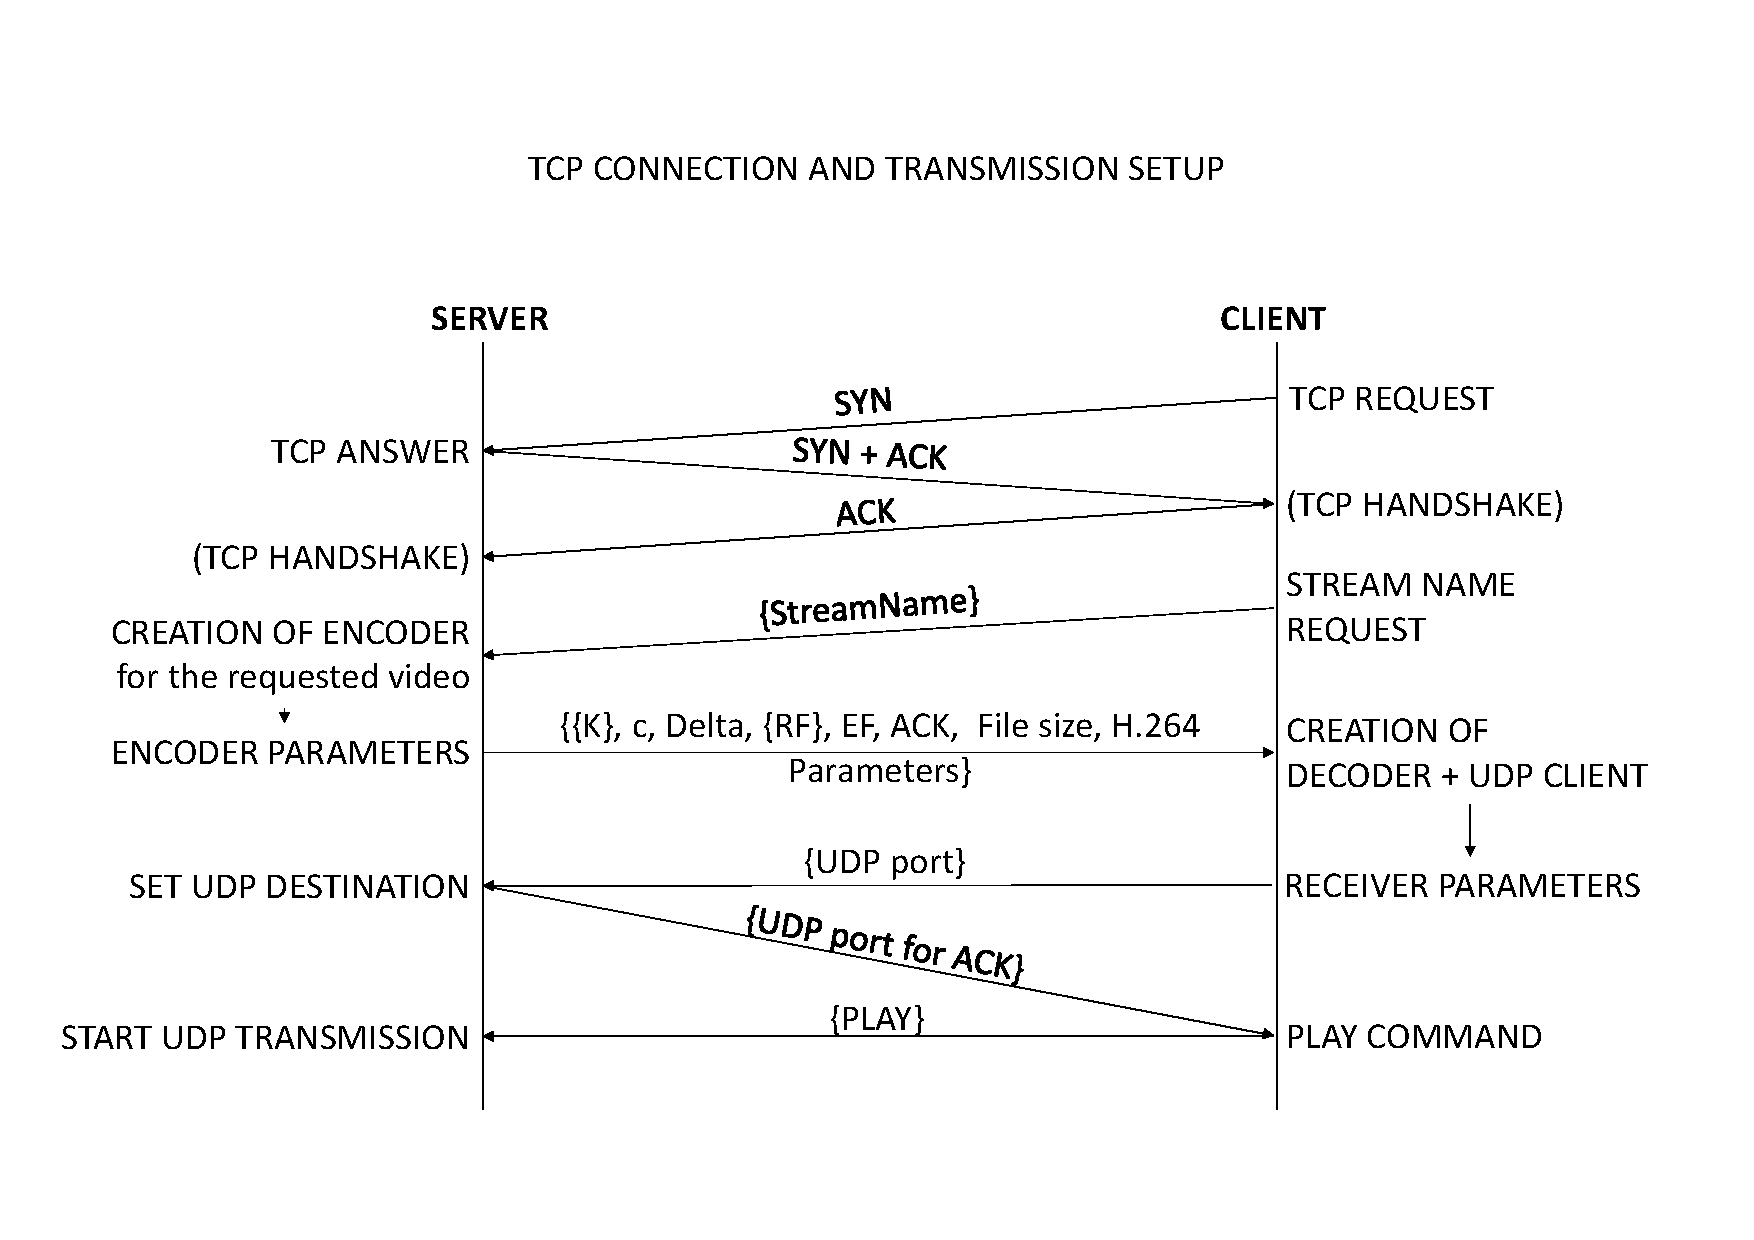
\includegraphics[trim=0cm 8cm 0cm 7cm, width=1.00\textwidth]{TCP.pdf}
%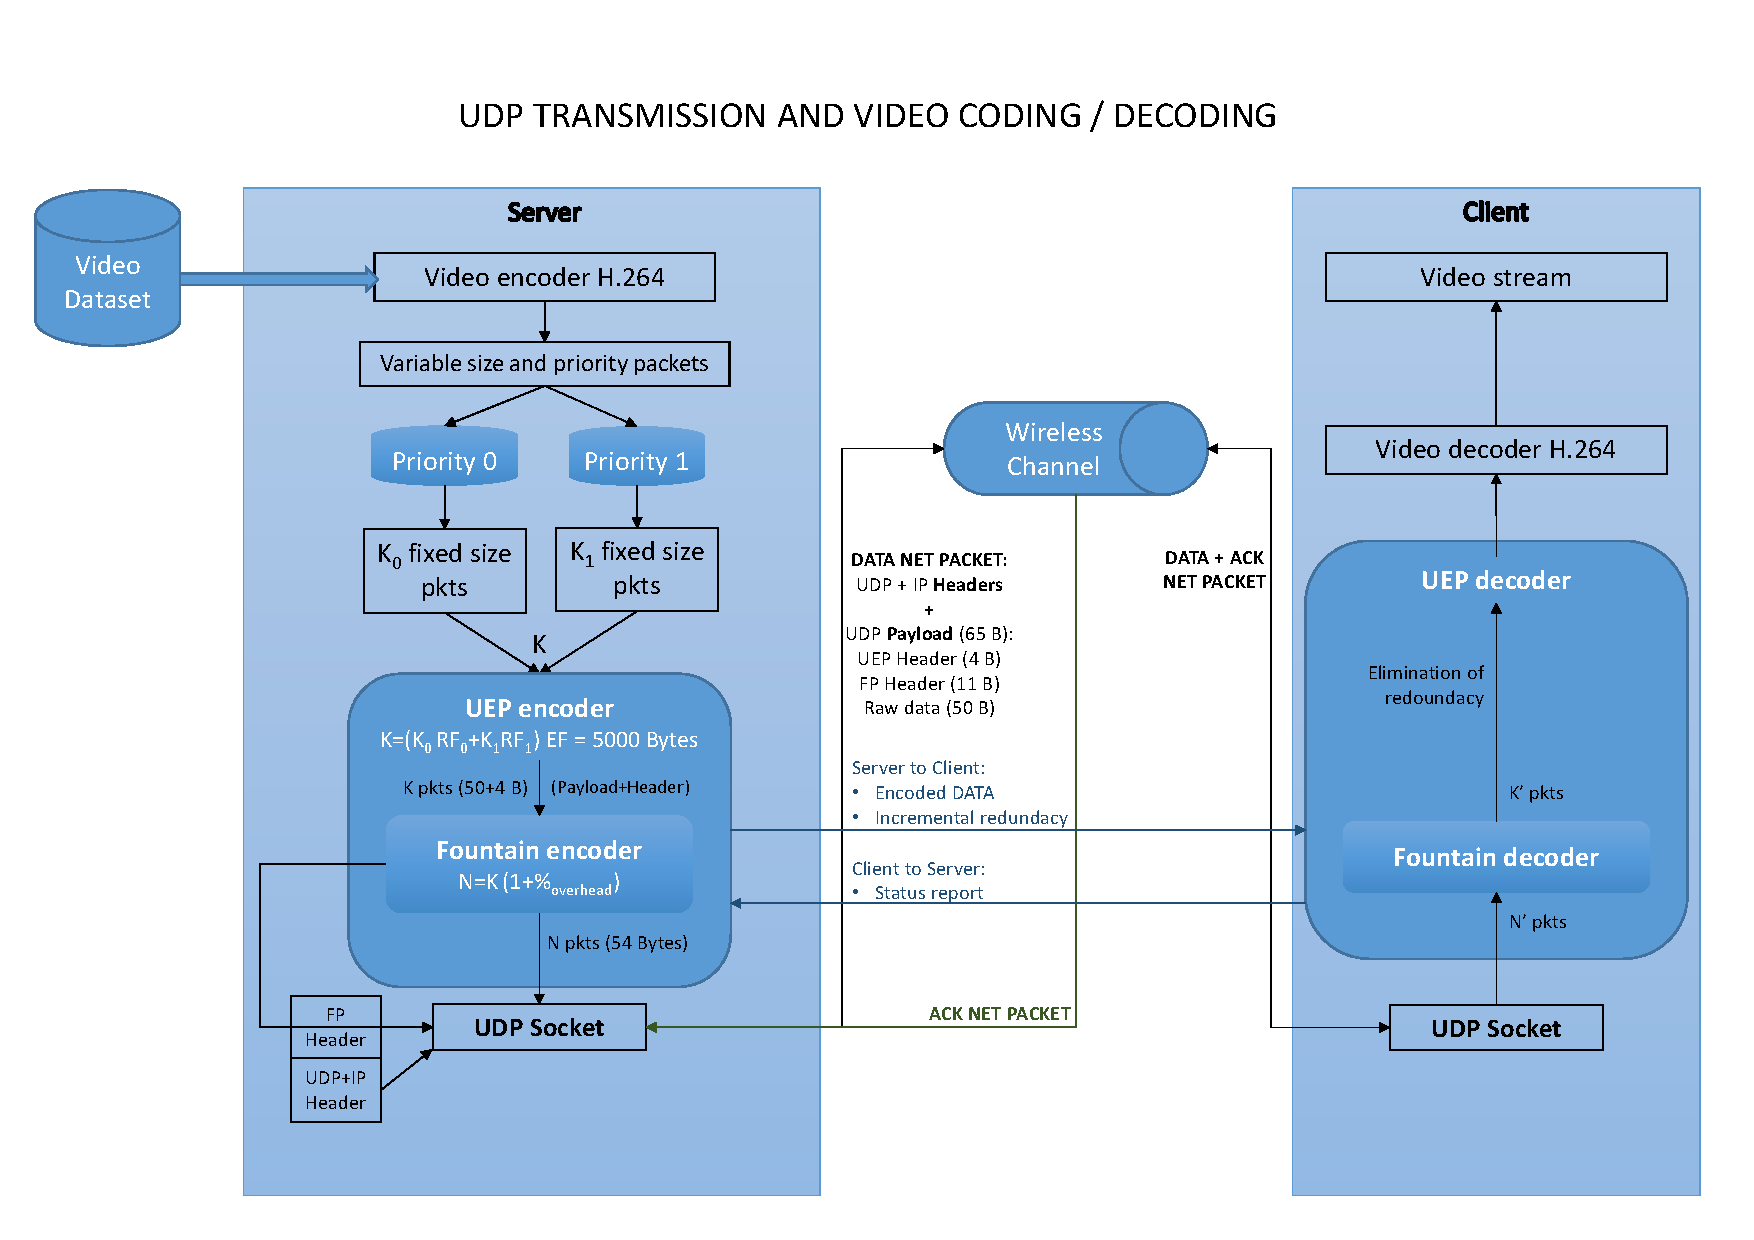
\includegraphics[width=180mm]{UDP.pdf}
%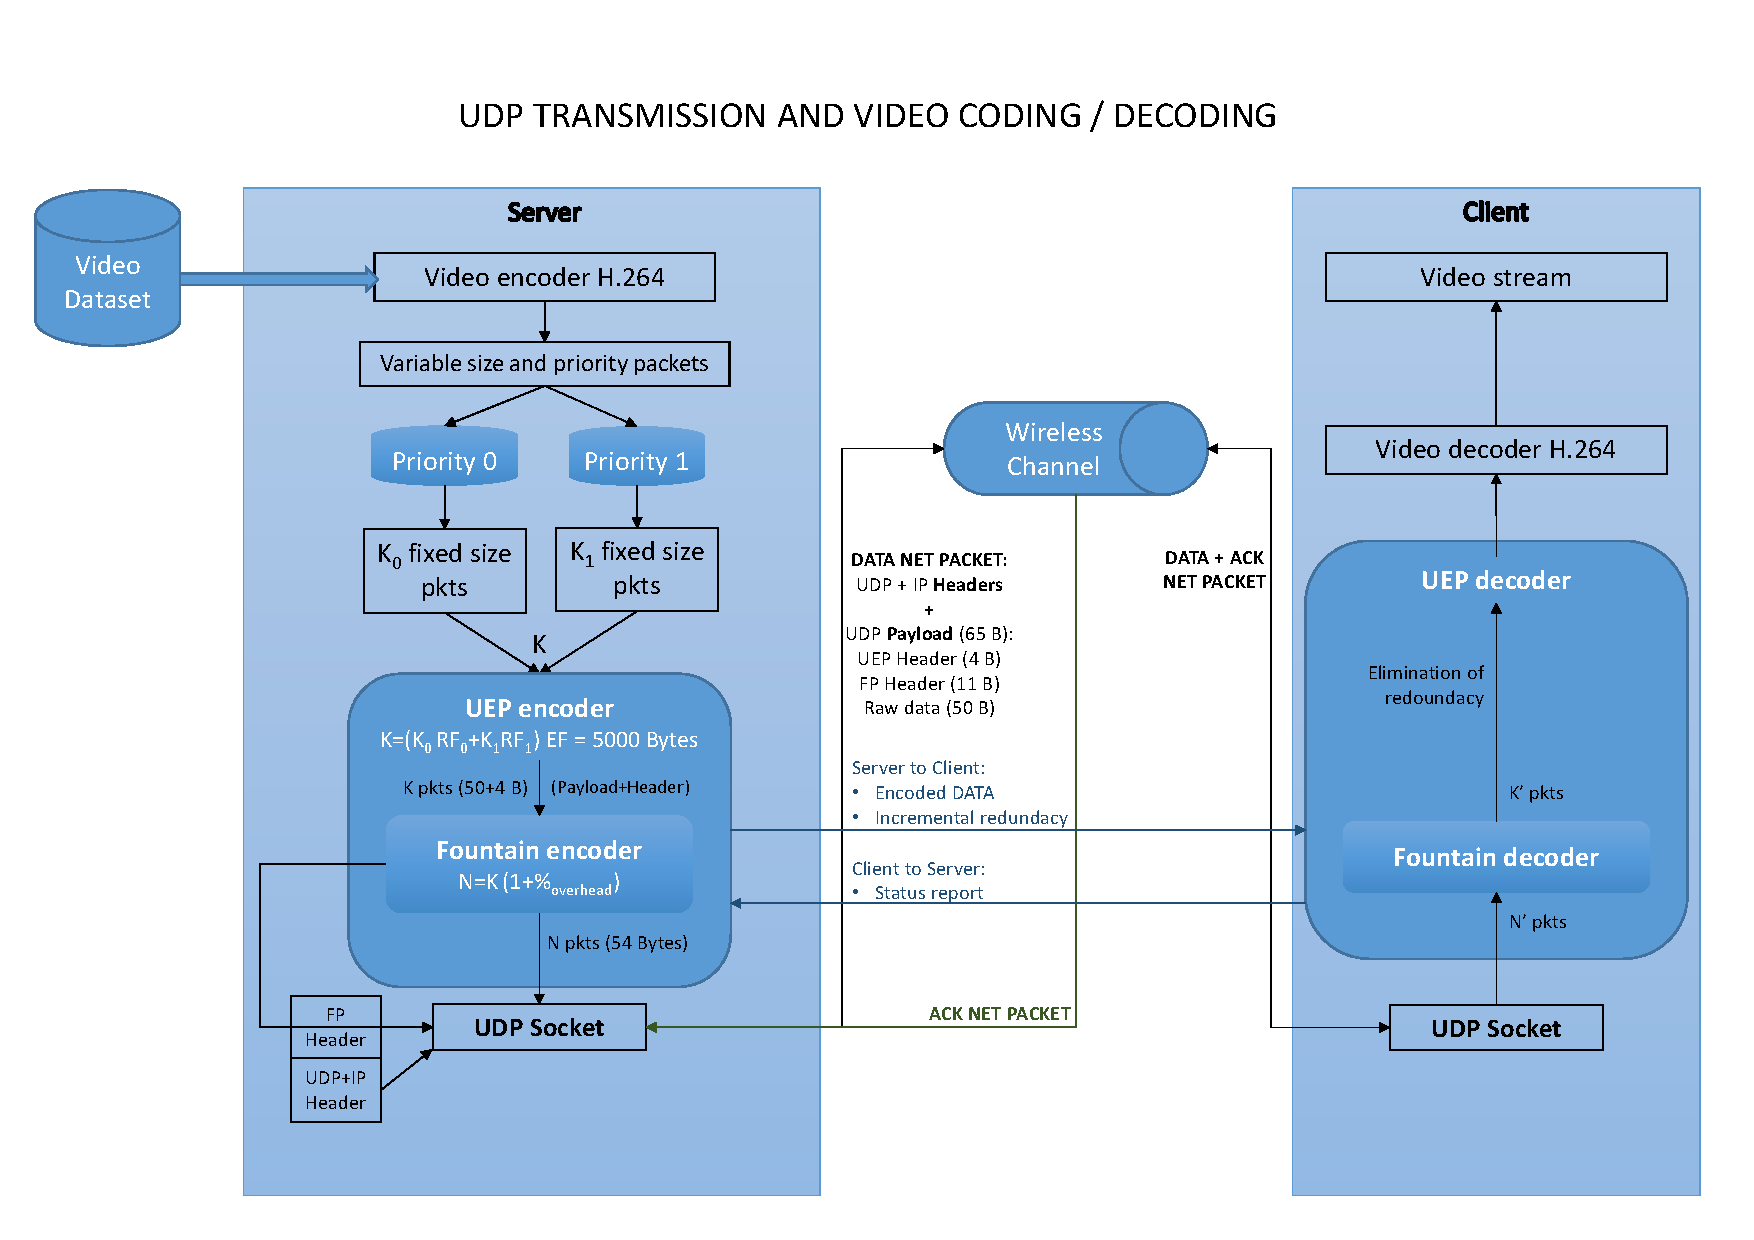
\includepdf[pages={1}]{UDP.pdf}
%\begin{figure}[htbp]
\begin{figure}[H]
    \centering
        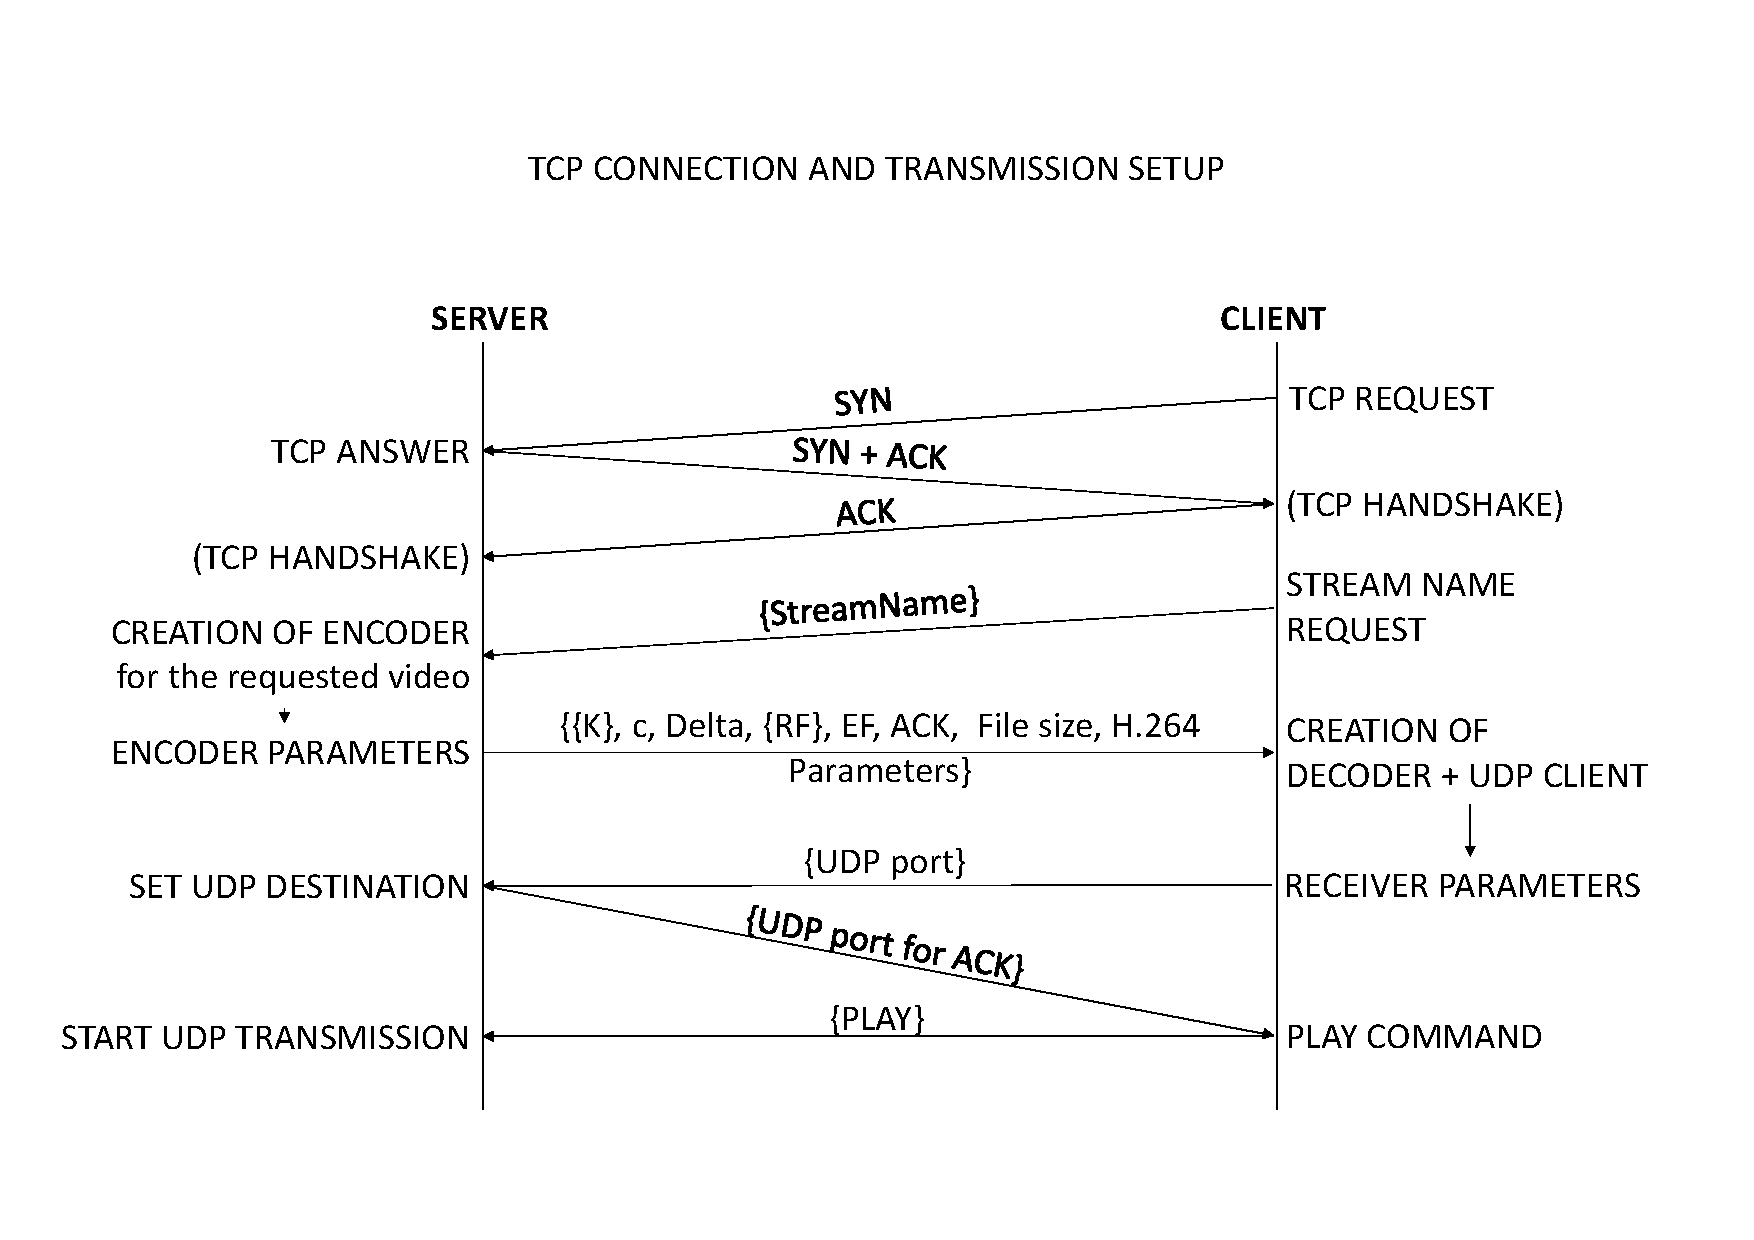
\includegraphics[clip, trim=0cm 1cm 0cm 1cm, width=1.00\textwidth]{TCP.pdf}
    \caption{TCP connection and tansmission setup}
    \label{fig:TCP}
\end{figure}
\begin{figure}[H]
    \centering
        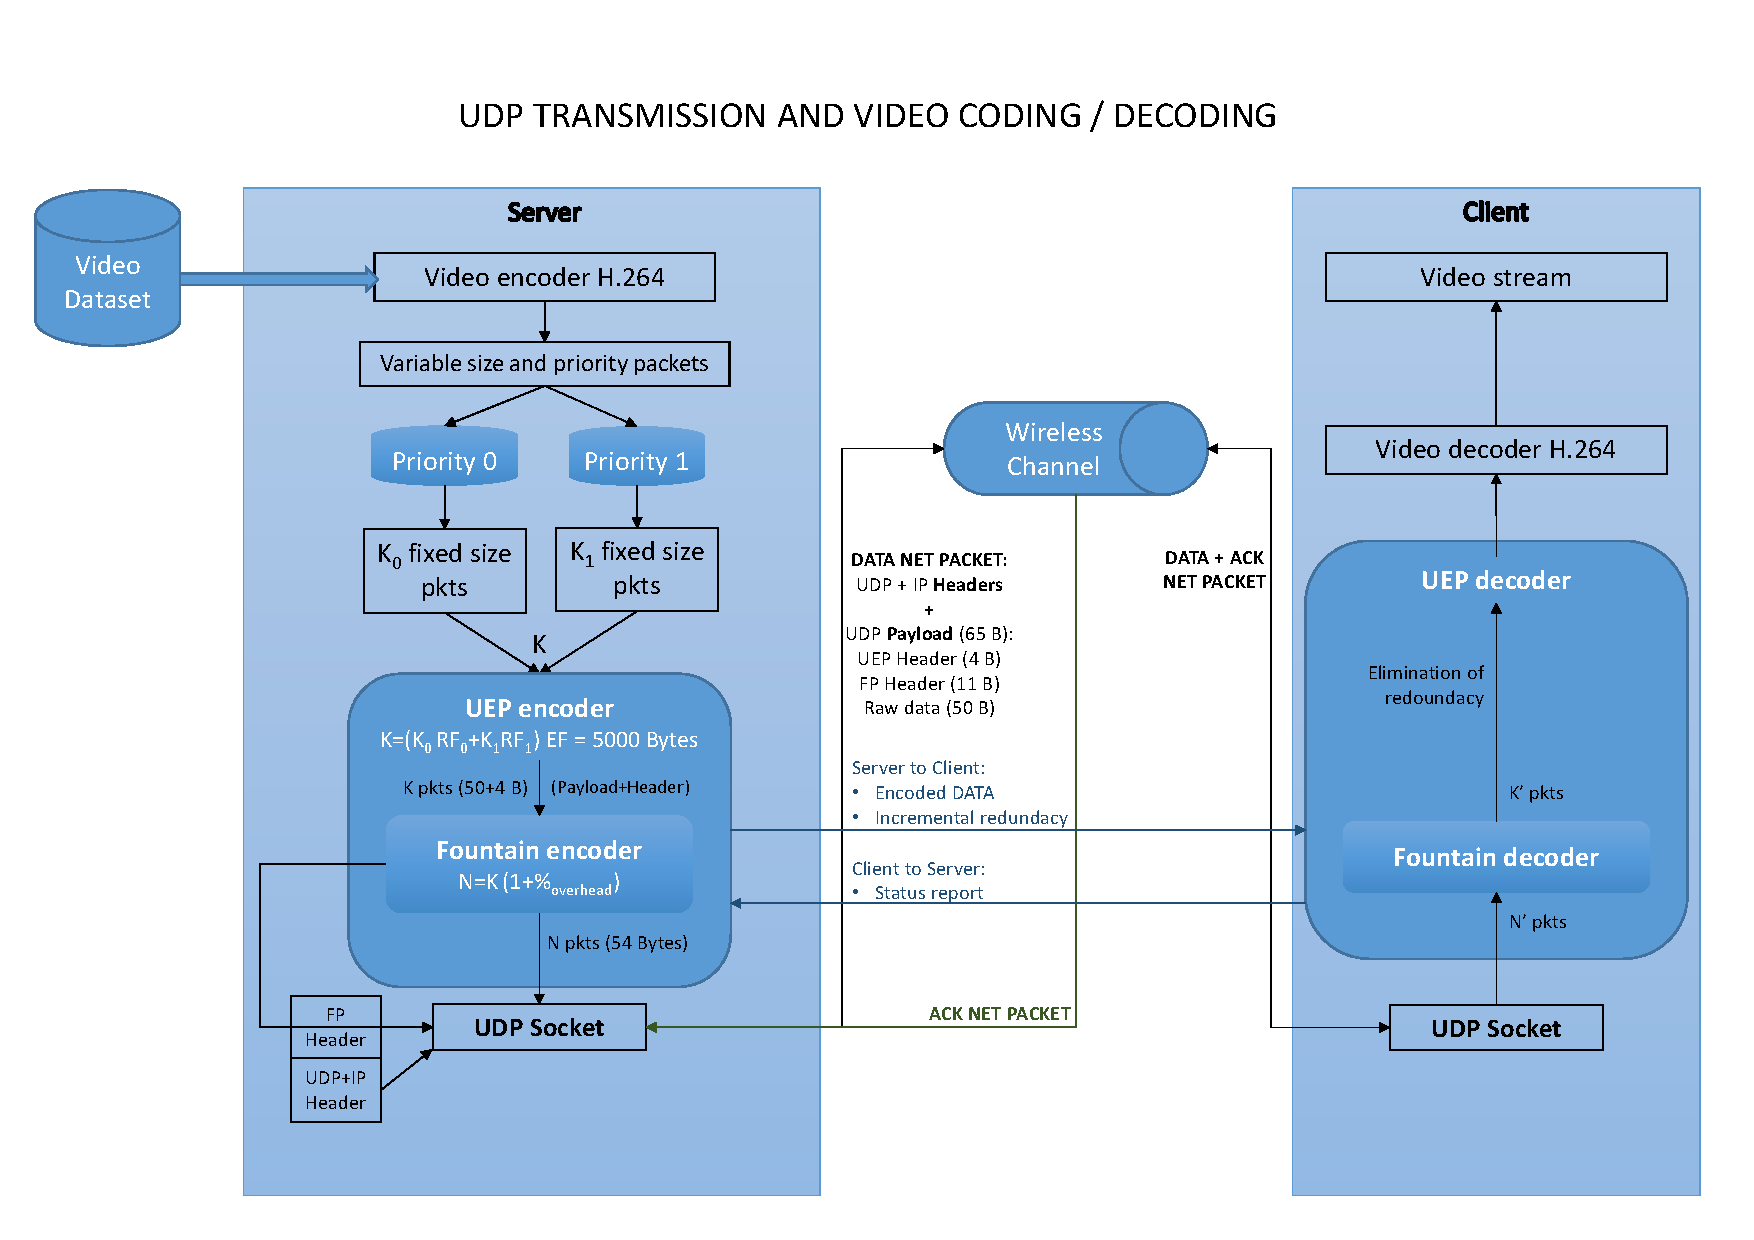
\includegraphics[clip, trim=0cm 1cm 0cm 1cm, width=1.00\textwidth]{UDP.pdf}
    \caption{Video stream encoding / decoding and transmission}
    \label{fig:UDP}
\end{figure}
%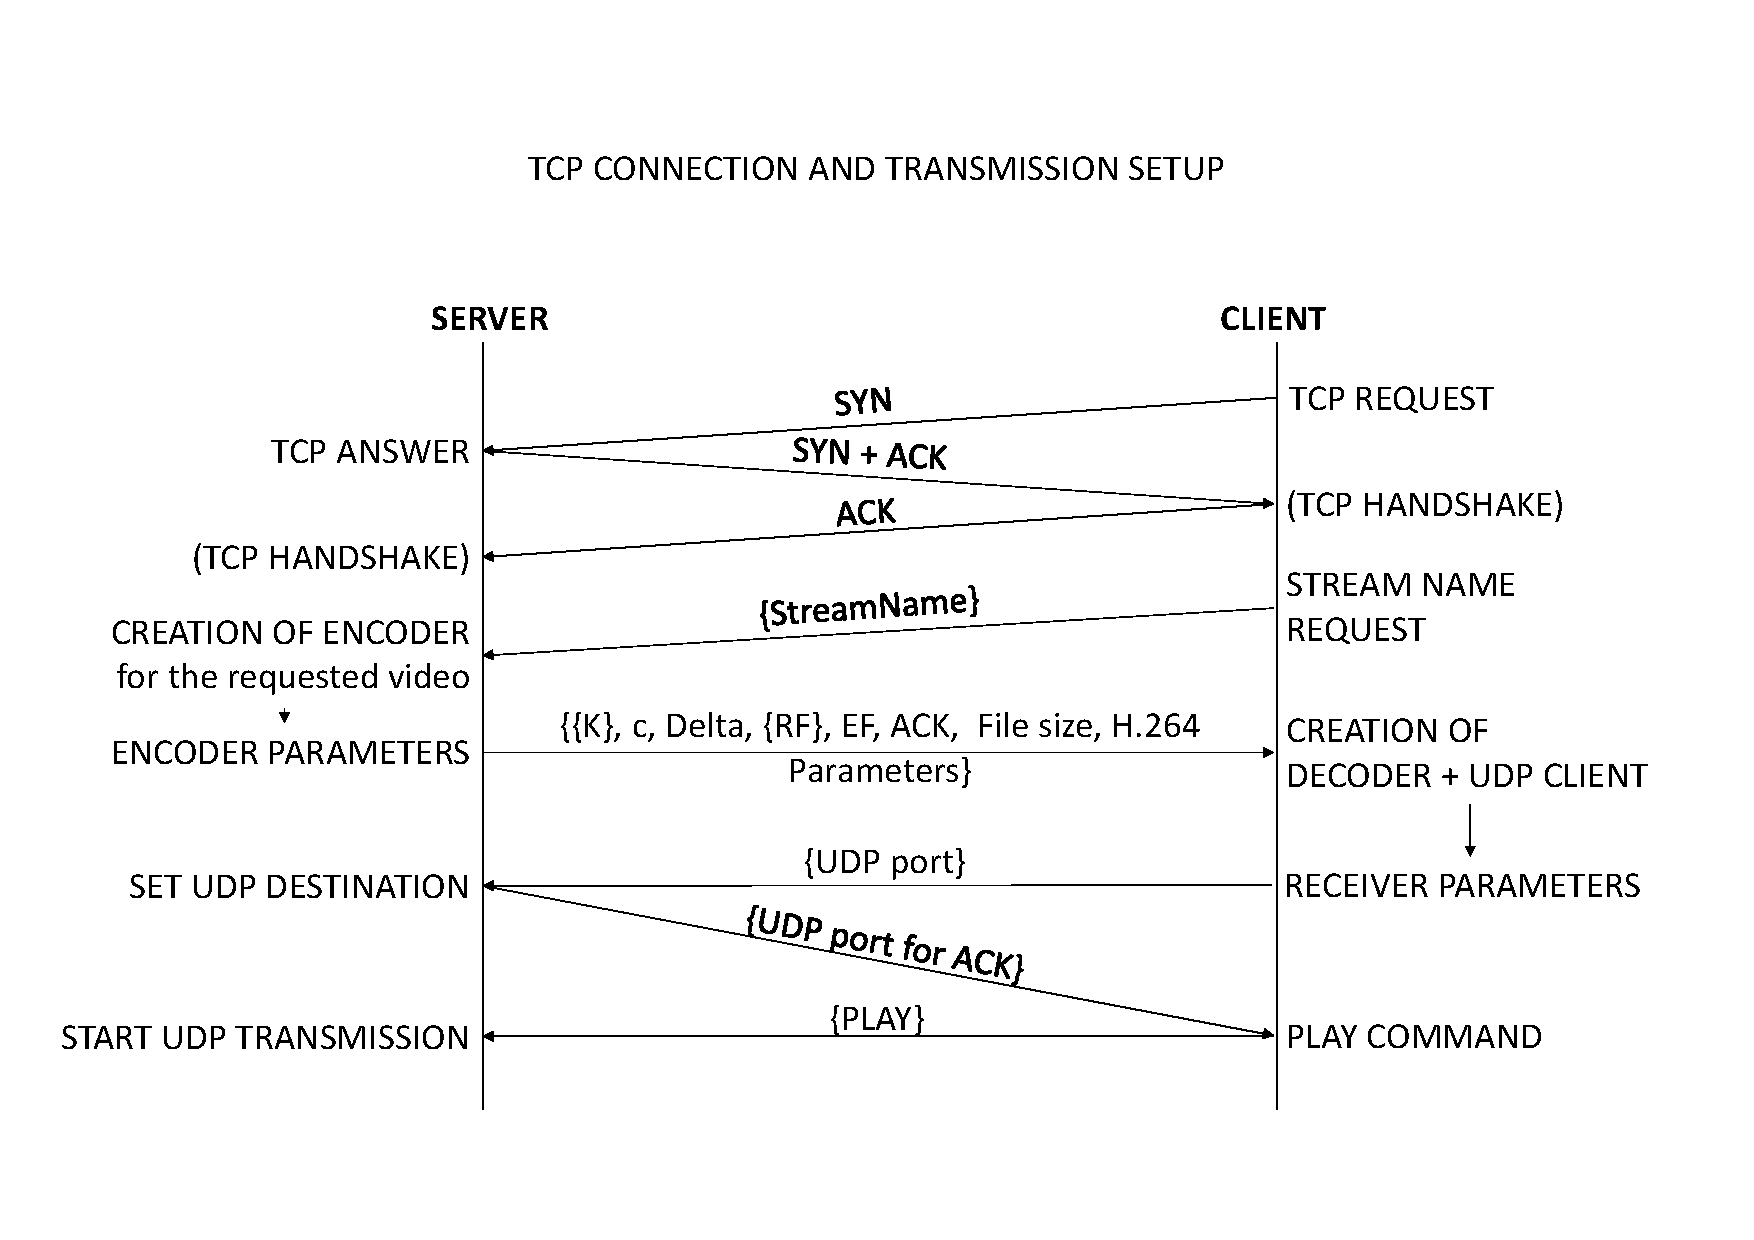
\includepdf{TCP.pdf}

\subsection{Modelli matematici}
\subsubsection{Canale}
Il canale è rappresentato da una catena di Markov a 2 stati: buono (G) e cattivo (B).\\
Sono stati effettuati test con due tipi di canale:
\begin{itemize}
\item Canale Markoviano, caratterizzato dalla seguente matrice di probabilità di transizione:\\
$$P=\begin{pmatrix}
1-p & p \\
q & 1-q
\end{pmatrix}$$
\item Canale senza memoria, con packet error rate fisso \textit{e}
\end{itemize}
Di seguito la rappresentazione Markoviana.
\begin{figure}[H]
    \centering
        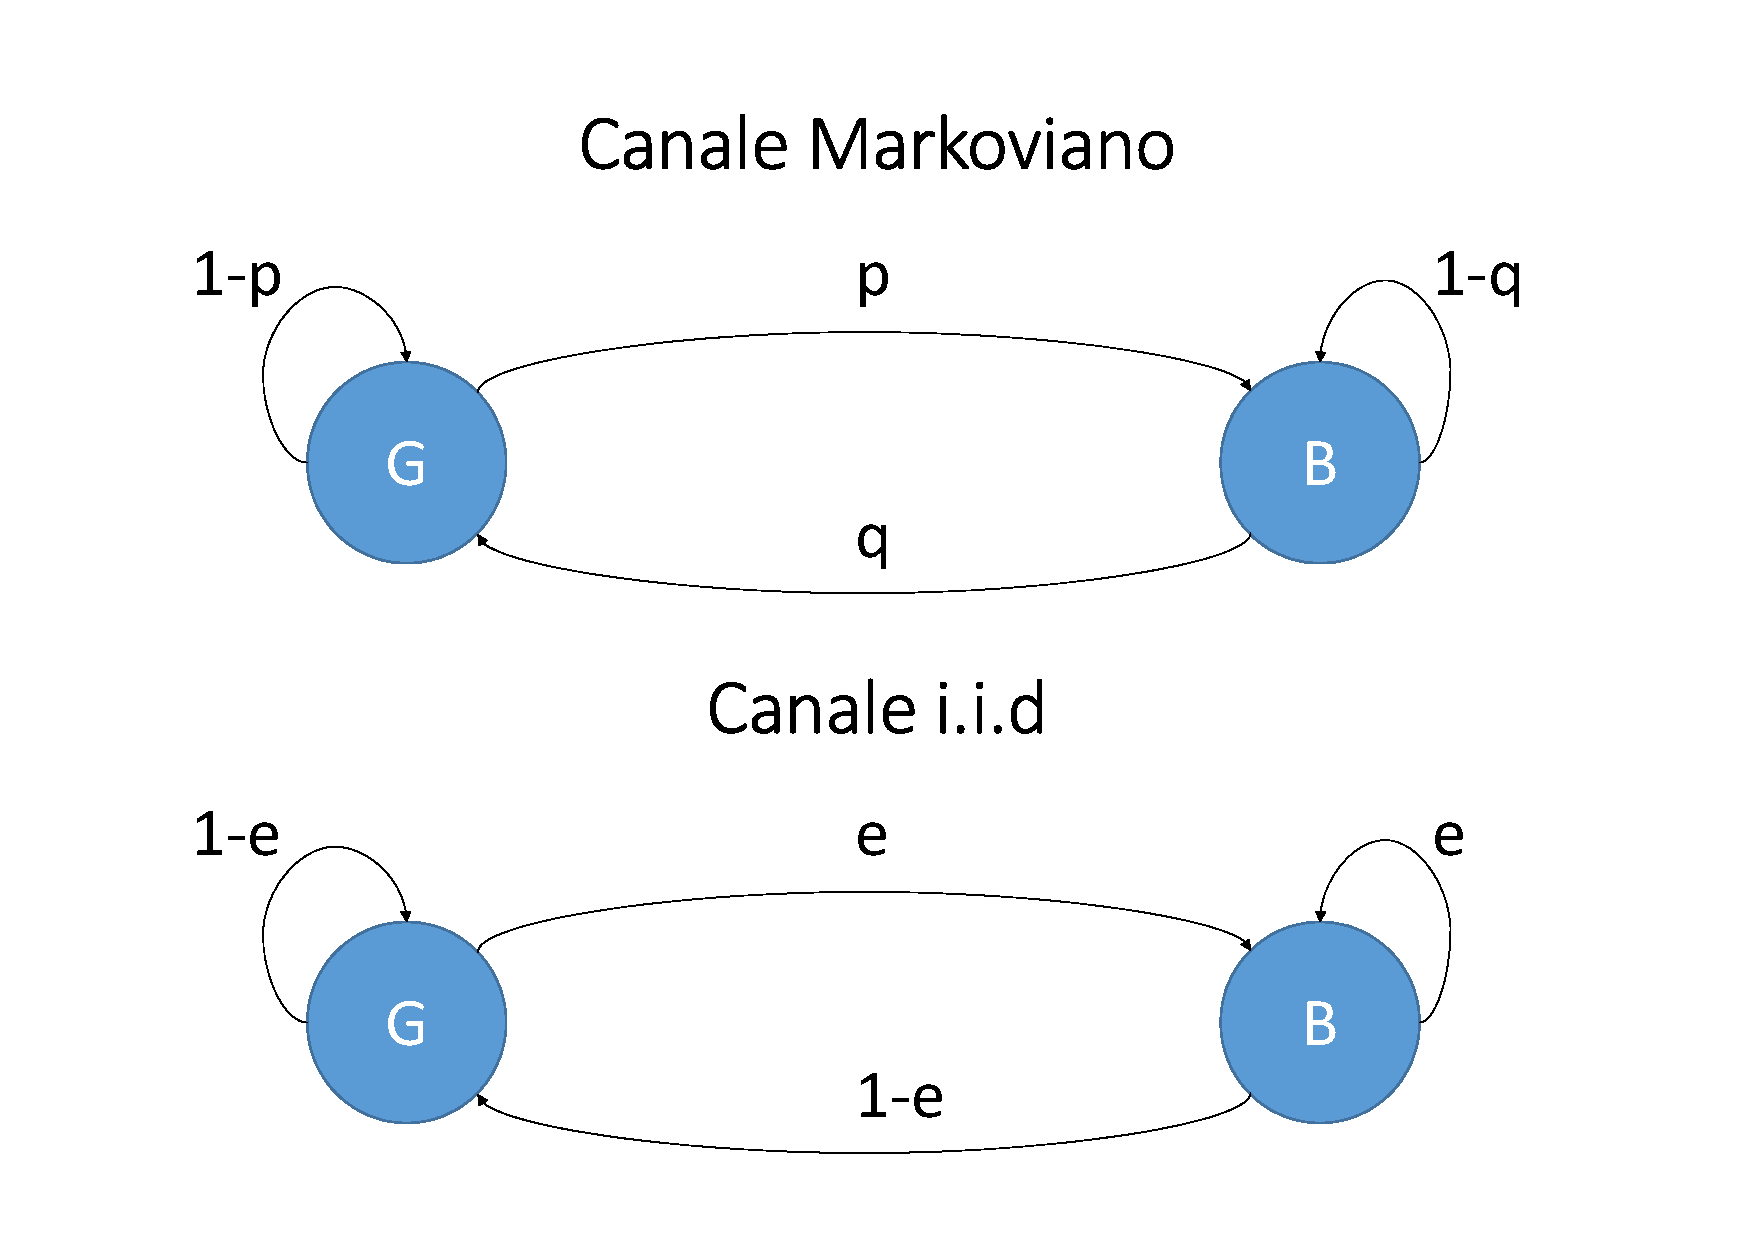
\includegraphics[clip, trim=0cm 1cm 0cm 1cm, width=0.5\textwidth]{Channel.pdf}
    \caption{Rappresentazione Markoviana dei due tipi di canale analizzati}
    \label{fig:Channel}
\end{figure}
\section{Risultati}

\section{Conclusioni}

\section{Bibliografia}
%\begin{figure}[H]
%	\makebox[\textwidth][c]{\includegraphics[width=16cm]{G10labE_f3.eps}}
%	\caption{Componenti di $\hat{s}$}\label{fig:s2}
%\end{figure}

\end{document}
